\documentclass[a4paper,french,bookmarks]{book}

\usepackage{booktabs}
\usepackage{minitoc}
\usepackage{Structure/4PE18TEXTB}
\usepackage{pdfpages}
\usepackage{tikz-3dplot}

\newboxans
\renewcommand{\questionsdecours}{\section*{\centering\EBGaramond\Large Questions~ de~ cours}}
\renewcommand{\thechapter}{\Roman{chapter}}
\renewcommand{\thesubsection}{Exercice \arabic{subsection}}
\setcounter{secnumdepth}{5}
\setcounter{tocdepth}{0}
\mtcsettitle{minitoc}{}
%\renewcommand{\thesection}{\hspace{-11pt}}
%\renewcommand{\thesubsection}{}

\newcommand{\chaptertoc}[0]{
    \setcounter{minitocdepth}{4}
    \begin{tcolorbox}[
        enhanced,
        frame hidden,
        sharp corners,
        detach title,
        spread outwards     = 5pt,
        halign              = center,
        valign              = center,
        borderline west     = {3pt}{0pt}{main20!50!main2!95!gray!90},
        coltitle            = main20!50!main2!95!gray!90, 
        interior style      = {
            left color      = main1white2!65!gray!11,
            middle color    = main1white2!50!gray!10,
            right color     = main1white2!35!gray!9
        },
        arc                 = 0 cm,
        title               = SOMMAIRE,
        fonttitle           = \bfseries\sffamily,
        overlay             = {
            \node[rotate=90, minimum width=1cm, anchor=south,yshift=-0.8cm] at (frame.west) {\tcbtitle};
        }
    ]
        \begin{minipage}{0.83\linewidth}
            \sffamily
            \minitoc
        \end{minipage}
    \end{tcolorbox}
}

\begin{document}
    
    %==============================
    % METADONNEES
    %==============================
    
    \title{TD de Physique de MPI/MPI* (2022-2023)}
    \author{SIAHAAN--GENSOLLEN Rémy}
    \date{\today}
    \hypersetup{
        pdftitle={TD de Physique de MPI/MPI* (2022-2023)},
        pdfauthor={SIAHAAN--GENSOLLEN Rémy},
        pdflang={fr-FR},
        pdfsubject={MPI/MPI*, TD de Physique},
        pdfkeywords={MPI/MPI*, TD de Physique, 2022-2023}
        pdfstartview=
    }
    
    %==============================
    % MISE EN PAGE
    %==============================
    
    \titleformat{\chapter}[display]{\normalfont\huge\bfseries}{}{0pt}{
        \begin{tcolorbox}[
            enhanced,
            frame hidden,
            sharp corners,
            spread sidewards    = 5pt,
            halign              = center,
            valign              = center,
            interior style      = {color=main3!20},
            arc                 = 0 cm,
            fontupper           = \color{black}\sffamily\bfseries\huge,
            fonttitle           = \normalfont\color{white}\sffamily\small,
            top                 = 1cm, 
            bottom              = 0.7cm,
            title               = Chapitre \thechapter,
            attach boxed title to bottom center = {
                yshift=\tcboxedtitleheight/2,
            },
            boxed title style = {
                frame code={
                \path[left color=main3!95!gray!90,right color=main3!95!gray!90] 
                    ([xshift=-10mm]frame.north west) -- 
                    ([xshift=10mm]frame.north east) -- 
                    ([xshift=10mm]frame.south east) -- 
                    ([xshift=-10mm]frame.south west) -- 
                    cycle;
                },
                interior engine=empty
            }
        ]
            #1
        \end{tcolorbox}%
    }
    \titlespacing*{\chapter}{0pt}{-120pt}{-15pt}
    \titleformat{name=\chapter,numberless}[display]{\normalfont\huge\bfseries}{}{0pt}{
        \begin{tcolorbox}[
            enhanced,
            frame hidden,
            sharp corners,
            spread sidewards    = 5pt,
            halign              = center,
            valign              = center,
            interior style      = {color=main3!20},
            arc                 = 0 cm,
            outer arc           = 0pt,
            leftrule            = 0pt,
            rightrule           = 0pt,
            fontupper           = \color{black}\sffamily\bfseries\huge,
            enlarge left by     = -1in-\hoffset-\oddsidemargin, 
            enlarge right by    = -\paperwidth+1in+\hoffset+\oddsidemargin+\textwidth,
            width               = \paperwidth, 
            left                = 1in+\hoffset+\oddsidemargin, 
            right               = \paperwidth-1in-\hoffset-\oddsidemargin-\textwidth,
            top                 = 1cm, 
            bottom              = 1cm
        ]
            #1
        \end{tcolorbox}%
    }
    \titlespacing*{name=\chapter,numberless}{0pt}{-115pt}{0pt}
    
    %==============================
    % PREMIERE DE COUVERTURE
    %==============================

    %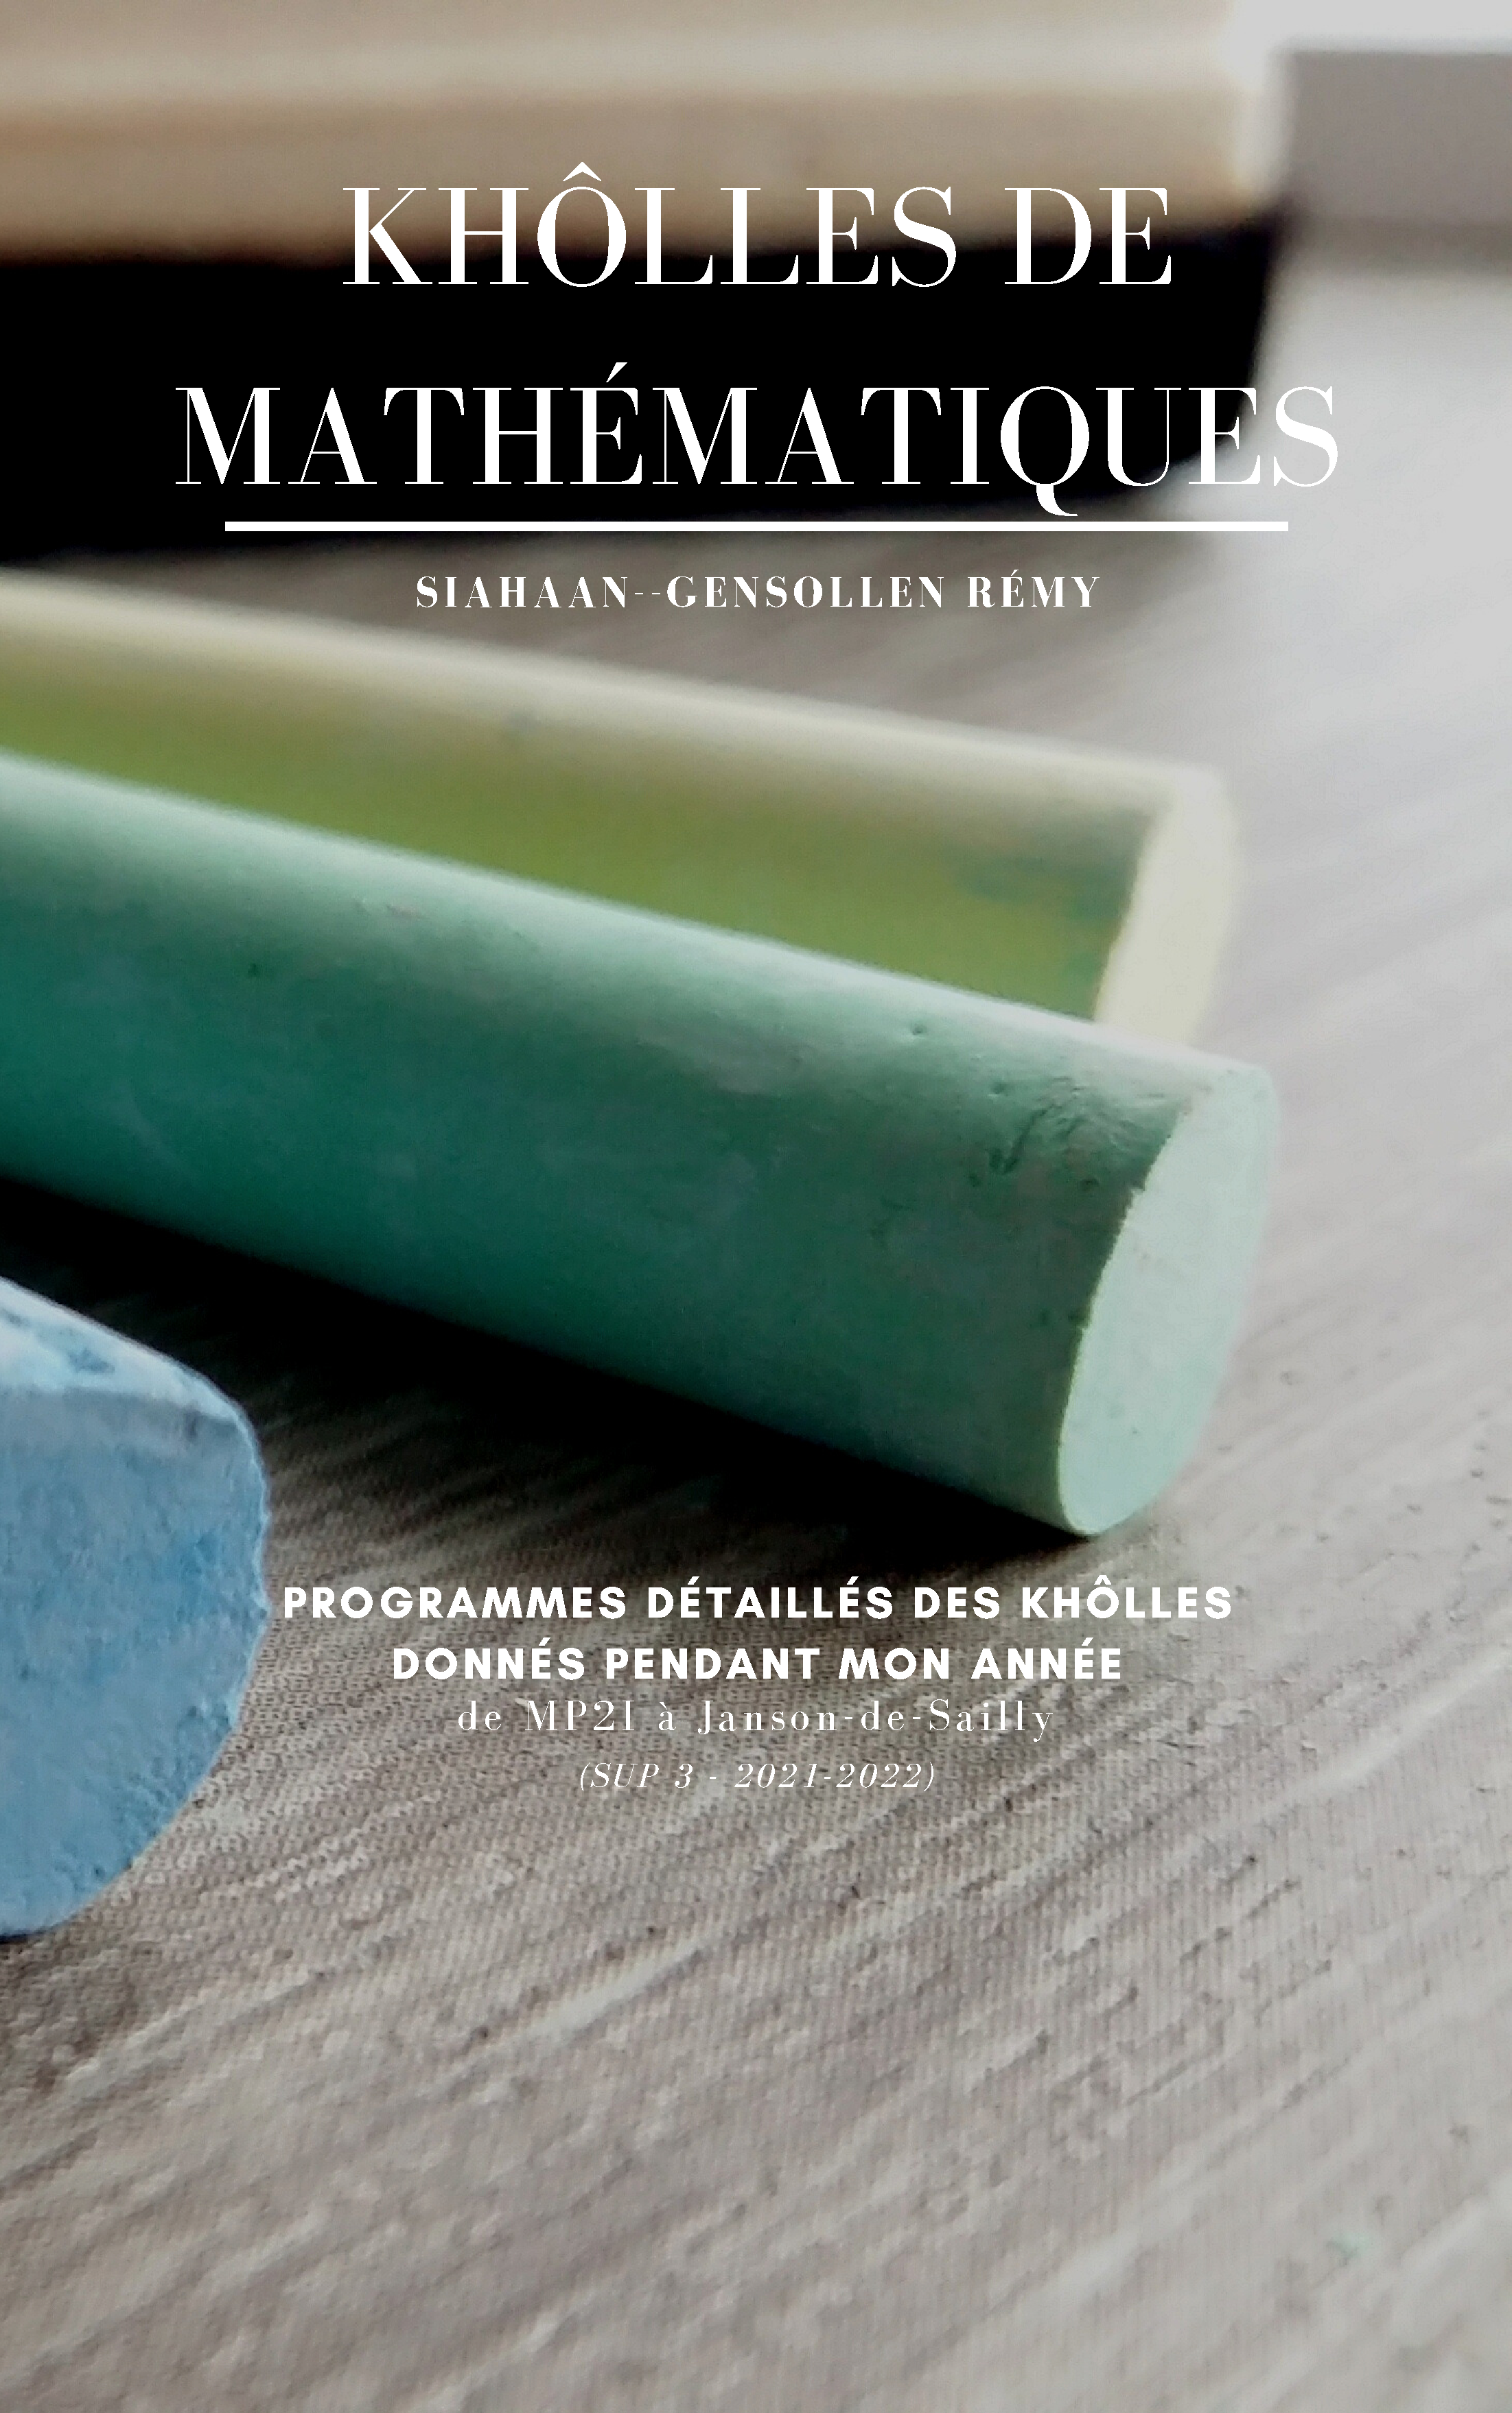
\includepdf[pages={1},scale=1.15,offset=0mm -18mm]{LDCCover.pdf}
    
    %==============================
    % PAGE VIDE
    %==============================
    
    %\pagestyle{empty}
    
    %==============================
    % PAGE DE COUVERTURE INTERNE
    %==============================
    
    \begin{titlepage}
	    \begin{center}
	        {\scshape SIAHAAN--GENSOLLEN Rémy\par}
	        \vspace{2cm}
	        {\huge\sffamily TD de\par}
	        \vspace{0.5cm}
	        {\Huge\bfseries\sffamily PHYSIQUE\par}
	        \vspace{1cm}
	        {\Large\textit{donné pendant mon année de \textsf{MPI/MPI*} à
	        Janson-de-Sailly}\\[5pt]\texttt{(2022-2023)}\par}
	        \vfill
	        {\large\EBGaramond Dernière compilation le \today\par}
        \end{center}
    \end{titlepage}
    
    %==============================
    % PAGE VIDE
    %==============================
    
    \pagestyle{empty}\text{}\newpage
    
    %==============================
    % STYLE DES EN-TÊTES ET PIEDS DE PAGES
    %==============================
    
    \renewcommand\chaptermark[1]{\markboth{#1}{}}
    
    \fancypagestyle{intro}{
        \fancyhf{}
        \renewcommand{\headrulewidth}{0pt}
        \renewcommand{\footrulewidth}{0pt}\fancyfoot[RO,LE]{\GillSansMTMedium\color{white5}\thepage\;/\;\pageref{LastPage}}
        \fancyhead[LE]{\GillSansMTMedium\color{white5}\bfseries TD DE PHYSIQUE}
        \fancyhead[RE]{\GillSansMTMedium\color{white5}Avant-propos}
        \fancyhead[LO]{\GillSansMTMedium\color{white5}\rightmark}
        \fancyhead[RO]{\GillSansMTMedium\color{white5}\textbf{MPI/MPI*} 2022-2023 \quad Janson-de-Sailly}
    }
    
    \fancypagestyle{toc}{
        \fancyhf{}
        \renewcommand{\headrulewidth}{0pt}
        \renewcommand{\footrulewidth}{0pt}\fancyfoot[RO,LE]{\GillSansMTMedium\color{white5}\thepage\;/\;\pageref{LastPage}}
        \fancyhead[LE]{\GillSansMTMedium\color{white5}\bfseries TD DE PHYSIQUE}
        \fancyhead[RE]{\GillSansMTMedium\color{white5}Table des matières}
        \fancyhead[LO]{\GillSansMTMedium\color{white5}\rightmark}
        \fancyhead[RO]{\GillSansMTMedium\color{white5}\textbf{MPI/MPI*} 2022-2023 \quad Janson-de-Sailly}
    }
    
    \fancypagestyle{plain}{
        \fancyhf{}
        \renewcommand{\headrulewidth}{0pt}
        \renewcommand{\footrulewidth}{0pt}\fancyfoot[RO,LE]{\GillSansMTMedium\color{white5}\thepage\;/\;\pageref{LastPage}}
        \fancyhead[LE]{\GillSansMTMedium\color{white5}\bfseries TD DE PHYSIQUE}
        \fancyhead[RE]{\GillSansMTMedium\color{white5}Chapitre \thechapter : \nouppercase{\leftmark}}
        \fancyhead[LO]{\GillSansMTMedium\color{white5}\nouppercase{\rightmark}}
        \fancyhead[RO]{\GillSansMTMedium\color{white5}\textbf{MPI/MPI*} 2022-2023 \quad Janson-de-Sailly}
    }
    
    %==============================
    % PREFACE 
    %==============================
    
    \chapter*{Avant-propos}
    \thispagestyle{intro}
    \addcontentsline{toc}{chapter}{Avant-propos}
    
    \text{\Large\EBGaramond\itshape À tout lecteur potentiel, quelques mots...}\newline\newline\newline
    
    \begin{center}
        \begin{minipage}{0.85\linewidth}
            \large \qquad Ce livre contient la résolution des exercices de TD donnés pendant les cours de physique de mon année de MPI/MPI*. Il vient en complément du livre de cours associé.\newline\newline\newline\text{}
        \end{minipage}
    \end{center}
    
    \hfill{\large\textsc{Siahaan--Gensollen Rémy}}
    
    \pagestyle{intro}
    
    %==============================
    % TABLE DES MATIERES
    %==============================
    
    \newpage
    \dominitoc\nomtcrule 
    {\sffamily\tableofcontents}\mtcaddchapter\pagestyle{toc}
    
    \cleardoublepage
    
    %==============================
    % COURS
    %==============================
    
    \pagestyle{plain}
    
    \chapter{Électrostatique}
    
    \begin{tcolorbox}[
        breakable,
        enhanced,
        frame hidden,
        interior style      = {fill = main3!10},
        sharp corners       = downhill,
        arc                 = 0 cm,
        boxrule             = 0 cm,
    ]
        \color{main3}{
            On rappelle l'expression du Laplacien en coordonnées sphériques, quand il y a une symétrie sphérique :
            %
            \[ \Delta f = \dfrac{1}{r}\dfrac{\partial^2 rf}{\partial r^2}\]
        }
    \end{tcolorbox}
    
    
    
    \subsection{Condensateur plan}
    
    Soit un condensateur plan dont les armatures sont des disques de surface $S$, séparés d'une distance $e$. Le milieu inter-armature est considéré comme équivalent au vide.
    
    \begin{enumerate}
        \item On impose une tension $V_0$ aux bornes du condensateur. Sachant que $e \ll \sqrt{S}$, quelle est la forme des lignes de champ dans l'espace inter-armature ? Justifier.
        
        \boxansconc{
            \begin{minipage}{0.65\linewidth}
                \begin{center}
                    \begin{tikzpicture}[cross/.style={path picture={
                        \draw[black] (path picture bounding box.south east) -- (path picture bounding box.north west) (path picture bounding box.south west) -- (path picture bounding box.north east);
                    }}]
                        \draw[<->] (0, -1) -- (0, 1) node[midway, left] {$e$};
                        
                        \draw[thick, main3] (0.4, 1) -- (5.4, 1) node[right] {$S_1$};
                        \draw[thick, main3] (0.4, -1) -- (5.4, -1) node[right] {$S_2$};
                        
                        \draw[-Latex, thick,main5] (4, -0.8) -- (4, 0.8);
                        
                        \node[main5] at (4.6, 0) {$V_0 > 0$};
                        
                        \draw[->] (6.7, 0.3) --++ (0.7, 0) node[right] {$\vec{e_x}$};
                        \draw[->] (6.7, 0.3) --++ (0, 0.7) node[right] {$\vec{e_z}$};
                        \node[draw,circle,cross,minimum width=0.3cm] at (6.7, 0.3){};
                        \node at (6.7, -0.15) {$\vec{e_y}$}; 
                    \end{tikzpicture}
                \end{center}
            \end{minipage}
            %
            \begin{minipage}{0.35\linewidth}
                On constante tout d'abord qu'on a les plans de symétrie
                %
                \[ \Pi_\text S\p{M, \vec{e_z}, \vec{e_x}} \qquad\et\qquad \Pi_\text S'\p{M, \vec{e_z}, \vec{e_y}} \]
            \end{minipage}
            %
            Ainsi, le champ $\vec E$ vérifie $\vec E\p{M} \in \Pi_\text S \cap \Pi_\text S'$, et est donc selon $\vec{e_z}$. On a ainsi $\vec E\p{M} = E\p{M}\vec{e_z}$. Par ailleurs, on a invariance par translation selon $\vec{e_x}$ et selon $\vec{e_y}$, d'où $\vec E\p{x, y, z} = E\p{z}\vec{e_z}$. On a bien montré que les lignes de champs sont des droites.
        }
        
        \item Déterminer la capacité de ce condensateur. Que vaut la densité surfacique de chaque en fonction de $V_0$ sur chacune des armatures ?
        
        \boxansconc{
            On a $C = \dfrac{Q_1}{V_1-V_2}$, donc on peut utiliser le \emph{théorème de \textsc{Gauss}} sur une armature isolée, puis \emph{le théorème de superposition}. Tout d'abord, on pose $S_G$ le cube de hauteur $2z$ (??) de sections $S$, ainsi le \emph{théorème de \textsc{Gauss}} livre
            %
            \[ \oiint_{S_G} \vec E \cdot \dif\vec S = \dfrac{Q_\text{int}}{\epsilon_0} \qquad\text{d'où}\qquad \niint_{\bsS_{G_1}}\vec E \cdot \dif\vec S + \niint_{\bsS_{G_2}}\vec E \cdot \dif\vec S + \niint_{\bsS_L} \vec E\cdot \dif \vec S = \dfrac{Q_\text{int}}{\epsilon_0} \]
            %
            en vertu de quoi on obtient $E\p{z}S - E\p{z}S + 0 = \dfrac{Q_\text{int}}{\epsilon_0} = \dfrac{\sigma S}{\epsilon_0}$. De plus
            %
            \[ \vec E\p{\mathfrak{sym}_{\Pi_\text S}\p{z}} = \mathfrak{sym}_{\Pi_\text S}\p{E\p{z}\vec{e_z}} \qquad\text{d'où ???}\qquad \vec{E}\p{-z} = E\p{z}\p{-\vec{e_z}}\]
            %
            donc $E\p{z} = \text{sgn}\p{z}\times\dfrac{\sigma}{\epsilon_0}$. Dès lors $E\p{z} = \left\lbrace\begin{array}{cl}
                0 & \text{si} \ z > e \ou z < 0\\
                \dfrac{-\sigma}{2\epsilon_0} &\text{si} \ 0\leq z\leq e
            \end{array}\right.$
            
            Finalement, on a $C = \dfrac{\sigma S}{\frac{\sigma e}{\epsilon_0}} = \dfrac{\epsilon_0 S}{e}$ et $\sigma = \dfrac{V_0\epsilon_0}{e}$.
        }
    \end{enumerate}
    
    On introduit dans l'espace inter-armature un disque d'épaisseur $e' < e$ et de section $S$, parallèlement aux armatures. Ce disque est constitué d'un matériau assimilé à un conducteur parfait globalement neutre dans lequel le champ électrique est nul.
    
    \begin{enumerate}[resume]
        \item Démontrer que la répartition de charge qui apparaît ne peux pas être surfacique. Donner les signes et relation entre les densités surfaciques des deux faces.

        \boxansconc{
            \begin{center}
                \begin{tikzpicture}[cross/.style={path picture={
                    \draw[black] (path picture bounding box.south east) -- (path picture bounding box.north west) (path picture bounding box.south west) -- (path picture bounding box.north east);
                }}]
                    \draw[<->] (-0.3, -1) -- (-0.3, 1) node[midway, left] {$e$};
                    \draw[<->] (0.2, -0.25) -- (0.2, 0.25) node[midway, left] {$e'$};
                    
                    \draw[thick, main3] (0.4, 1) -- (5.4, 1) node[right] {$\sigma, V_1$};
                    \draw[thick, main3] (0.4, -1) -- (5.4, -1) node[right] {$-\sigma, V_2$};
                    
                    \fill[main3!30] (0.4, -0.2) rectangle (5.4, 0.2);
                    
                    \draw[thick, main3!40] (0.4, 0.25) -- (5.4, 0.25) node[right,main3] {$-\sigma'$};
                    \draw[thick, main3!40] (0.4, -0.25) -- (5.4, -0.25) node[right,main3] {$\sigma'$};
                    
                    \draw[->] (6.7, 0.3) --++ (0.7, 0) node[right] {$\vec{e_x}$};
                    \draw[->] (6.7, 0.3) --++ (0, 0.7) node[right] {$\vec{e_z}$};
                    \node[draw,circle,cross,minimum width=0.3cm] at (6.7, 0.3){};
                    
                    \node[fill=main3,circle,inner sep=1pt,label={[font=\footnotesize,main3]south east:$A$}] at (3, 1){};
                    \node[fill=main3,circle,inner sep=1pt,label={[font=\footnotesize,main3]east:$B$}] at (3, 0.25){};
                    \node[fill=main3,circle,inner sep=1pt,label={[font=\footnotesize,main3]east:$C$}] at (3, -0.25cm){};
                    \node[fill=main3,circle,inner sep=1pt,label={[font=\footnotesize,main3]north east:$D$}] at (3, -1cm){};
                    
                    \node at (6.7, -0.15) {$\vec{e_y}$}; 
                \end{tikzpicture}
            \end{center}
            %
            On a $\vec E=0$ dans le disque donc $\vec \nabla \cdot \vec E = \sigma$. Or $\vec \nabla \cdot \vec E = \dfrac{e}{\epsilon_0}$ d'où $e = \sigma$. Ainsi, une accumulation de charges elle ne peut être que surfacique. De plus $\sigma_1 = -\sigma_2$ par conservation de la charge et $\sigma_1>0$ car les électrons sont attirés par le plus haut potentiel.

        }
        
        \item Que vaut la capacité du condensateur en présence du disque ?
        
        \boxansconc{
            Or $\vec E_\text{int} = \vec 0$ d'où $\dfrac{-\sigma}{\epsilon_0} + \dfrac{\sigma'}{\epsilon_0} = 0$. Donc :
            %
            \begin{align*}
                V_1 - V_2 &= \int_A^D \vec E \cdot \dif\vec e = \int_A^B \vec E \cdot \dif\vec e + \int_B^C \vec E \cdot \dif\vec e +  \int_C^D \vec E \cdot \dif\vec e\\
                &= \dfrac{-\sigma}{\epsilon_0} \int_A^B \vec{e_z}\dif z\p{-\vec{e_x}} + 0 + \dfrac{-\sigma}{\epsilon_0}\int_C^D \vec{e_z}\dif z\p{-\vec{e_z}}\\
                &= \dfrac{\sigma}{\epsilon_0}\p{e-e_q-e'} + \dfrac{\sigma}{\epsilon_0}e_q = \dfrac{\sigma}{\epsilon_0}\p{e-e'}
            \end{align*} 
            %
            On a finalement $C = \dfrac{Q_S}{V_1 - V_2} = \dfrac{\sigma S}{\frac{\sigma}{\epsilon_0}\p{e - e'}} =\dfrac{\epsilon_0 S}{e - e'}$
        }
    \end{enumerate}
    
    \subsection{Potentiel}
    
    On donne le potentiel électrostatique $V\p{r} = \dfrac{Q}{4\pi \epsilon_0 r}\exp{-\dfrac{r}{r_0}}$ en coordonnées sphériques.
    
    \begin{enumerate}
        \item Calculer en tout point autre que $O$ la densité de charge $\rho\p{r}$.
        
        \boxansconc{
            On a $\vec \nabla \cdot \vec E = \vec \nabla \cdot \p{-\vec \nabla V} = - {\vec \nabla}^2 V = -\Delta V = \dfrac{\rho}{\epsilon_0}$. Or
            %
            \[ \Delta V = \dfrac{1}{r}\dfrac{\partial^2 rV\p{r}}{\partial r^2}= \dfrac{1}{r}\dfrac{Q}{4\pi\epsilon_0r_0^2}\exp{-\dfrac{r}{r_0}}\]
            %
            Et $\dfrac{-\rho\p{r}}{\epsilon_0} = \vec \nabla \cdot \vec E$, d'où l'on a $\rho\p{r} = -\dfrac{Q}{4\pi r_0^2}\dfrac{1}{r}\exp{-\dfrac{r}{r_0}}$
        }
        
        \item Calculer la charge à l'intérieur d'une sphère de rayon $R$ centrée en $O$.

        \boxansconc{
            On a $\rho\p{M} = \dfrac{\dif Q_{\dif V}}{\dif V}$
            \[Q'=\iiint_V\rho\p{r}\dif\tau=\int_0^R\rho(r)r^2\dif r\int_0^{2\pi}\sin\p{\theta}\dif\theta\int_0^{2\pi}\dif\varphi = -Q+Q\exp\p{\dfrac{-R}{r_0}}\p{\dfrac{R}{r_0}-1}\]
            D'autre part on a $Q_\text{int} = Q'+Q_0 = \epsilon_0E(r)4\pi r^2$ d'après le théorème de \textsc{Gauss}.
        }
        
        \item En déduire la présence en $O$ d'une charge que l'on déterminera.
        
        \boxansconc{
            On a $Q_0 = \lim\limits_{r \to 0} Q_\text{int}\p{r}$, d'où $Q_0 = Q$.
        }
        
        \item Calculer la charge totale de l'espace et la charge de l'espace privée du point $O$.
        
        \boxansconc{
            On a $Q_\text{total} = Q + \lim\limits_{r \to +\infty} Q_\text{int}\p{r}$. On a donc une distribution volumique négative dans tout l'espace, dont la somme vaut $-Q$.
        }
        
        \item Étudier la densité radiale de charge $4\pi r^2\rho\p{r}$.
        
        \boxansconc{
            On a $\dfrac{\dif q}{\dif r}$ ....
        }
    \end{enumerate}
    
    \subsection{Dsitrubution volumique}
    
    Soit la distribution volumique de charge $\rho = \rho_0\exp\p{-\dfrac{\mod{z}}{\delta}}$. Déterminer le champ électrique en tout point de l'espace.
    
    \boxansconc{
        On a les plans de symétries
        %
        \[ \Pi_\text S\p{M, \vec{e_x}, \vec{e_z}} \qquad\et\qquad Pi_\text S'\p{M, \vec{e_y}, \vec{e_z}} \]
        %
        d'où $\vec E\p{M} = E\p{M}\vec{e_z}$. On a de plus invariance par translation selon $\vec{e_x}$ et selon $\vec{e_y}$, d'où
        %
        \[ \vec E\p{x, y, z} = E\p{z}\vec{e_z} \]
        %
        De plus $\vec \nabla \cdot \vec E =\dfrac{\rho}{\epsilon_0}$ donc
        %
        \[\dfrac{\partial E_z}{\partial z}=\dfrac{\rho_0}{\epsilon_0}\exp\p{\frac{-\left|z\right|}{\delta}}\]
    }
    
    \subsection{Électrode hyperboloïde}
    
    \begin{minipage}{0.6\linewidth}
        On étudie le champ électrique créé par un dispositif constitué de trois électrodes :
        %
        \begin{enumerate}
            \itt une électrode en forme d'hyperboloïde de révolution autour de l'axe $\p{Oz}$, portée au potentiel $V_0$ et dont les sommets sont distants de $R$ de $O$.
            
            \itt deux calottes dont les sommets se situent en $z = \pm h$ de potentiel nul.
        \end{enumerate}
        %
        La situation est représentée sur le schéma ci-contre.
    \end{minipage}
    %
    \begin{minipage}{0.4\linewidth}
        
    \end{minipage}
    
    \begin{enumerate}
        \item On écrit le potentiel électrique $V$ au voisinage de $O$ à l'aide d'un développement limité à l'ordre $2$ :
        %
        \[ V = a + bx + cy + dz + ex^2 + fy^2 + gz^2 + ixy + jxz + kyz\]
        %
        Déterminer $a$, $b$, $c$, $d$, $e$, $f$, $g$, $i$, $j$ et $k$. En déduire le champ électrique au voisinage de $O$.
        
        \item On place un électron en $O$, est-il à l'équilibre ? Discuter de la stabilité axiale et radiale.
    \end{enumerate}
    
    \subsection{Charge dans un milieu ionisé}
    
    Une charge $Q > 0$ est placée dans un milieu ionisé. Pour résoudre l'équation de \textsc{Poisson}, on supposera que les charges suivent une distribution de \textsc{Boltzmann} : la probabilité qu'une particule soit dans un état d'énergie $\bsE$ est proportionelle à $\exp{-\frac{\bsE}{kT}}$. On utilisera l'approximation haute température.
    
    \begin{enumerate}
        \item Le milieu ionisé est un plasma de particules chargées $+q$ et $-q$ mobiles, de densité volumique $n_0$.
        
        \boxansconc{
            \begin{minipage}{0.5\linewidth}
                \begin{center}
                    \begin{tikzpicture}
                        \draw[thick, -latex,main3] (0, 0) -- ({sqrt(2)}, {-sqrt(2)}) node[midway, right] {$r$};
                        
                        \node[fill=black,circle,inner sep=1pt,label={left:$O$}] at (0,0){};
                        
                        \draw[main3,densely dotted,thick] (0, 0) circle (2);
                    \end{tikzpicture}
                \end{center}
            \end{minipage}
            %
            \begin{minipage}{0.5\linewidth}
                On a $\rho = \dfrac{\dif Q_\text{int}}{\dif \tau} = \dfrac{\dif N_+ q}{\dif \tau} + \dfrac{\dif N_-\p{-q}}{\dif \tau} = q\p{n_+ -n_-}$.
                
                Par \emph{théorème de liaison}, on a $\Delta V = -\dfrac{\rho}{\epsilon_0}$.
                
                GROS MORCEAU MANQUANT
            \end{minipage}
            %
            \[ \Delta V = \dfrac{2qn_0}{\epsilon_0}\sh{\dfrac{qVr}{kT}} \eq{\text{approx.}\ T \gg 1} \dfrac{2qn_0}{\epsilon_0}\dfrac{qV}{kT} \qquad\text{donc}\qquad \dfrac{1}{r}\dfrac{\partial^2 rV}{\partial r^2} - \dfrac{2q^2n_0}{\epsilon_0 kT}V = 0\]
            %
        }
        
        \item Résoudre l'équation différentielle en posant $U = rV$.
        
        \boxansconc{
            En posant $U = rV$, on a $\dfrac{\dif^2 U}{\dif r^2} - \dfrac{U}{r_0^2} = 0$, avec $r_0^2 = \dfrac{\epsilon_0 kT}{2q^2n_0}$, d'où l'on a 
            %
            \[ U\p{r} = Ae^{\sfrac{r}{r_0}} + Be^{-\sfrac{r}{r_0}} \qquad\text{donc}\qquad V\p{r} = A\dfrac{e^{\sfrac{r}{r_0}}}{r} + B\dfrac{e^{\sfrac{r}{r_0}}}{r}\]
            %
            Lorsque $r$ tend vers $+\infty$, ona $\lim\limits_{r \to +\infty} V\p{r} = 0$ d'où $A = 0$. Par ailleurs, lorsque $r$ tend vers $0$,  on a 
            %
            \[ V\p{r} \asymp{0} V_Q\p{r} = \dfrac{Q}{4\pi\epsilon_0 r} \qquad\et\qquad V\p{r} \asymp{0} B\dfrac{1 - \sfrac{r}{r_0}}{r} \asymp{0} \dfrac{B}{r} \qquad\text{donc}\qquad B = \dfrac{Q}{4\pi \epsilon_0}\]
        }
        
        \item Justifier l'approximation haute température.
    \end{enumerate}
    
    \subsection{Tunnel dans la Terre}
    
    \begin{minipage}{0.7\linewidth}
        Un tunnel rectiligne est percé dans la terre comme indiqué sur le schéma ci-contre. La Terre est supposée à symétrie sphérique de masse volumique $\rho$ et on admettra que le tunnel ne perturbe pas son champ de gravitation. Une bille de masse $m$ peut glisser sans frotter dans le tunnel, étudier son mouvement.
    \end{minipage}
    %
    \begin{minipage}{0.3\linewidth}
        \begin{center}
            \begin{tikzpicture}[scale=1.5]
                 \node[fill=black,circle,inner sep=1pt,label={left:$O$}] at (0,0){};
                        
                \draw[main3,thick] (0, 0) circle (1);
                
                \fill[white] (-1, 0.65) rectangle (1, 0.80);
                \draw[main3,thick] (-0.76, 0.65) -- (0.76, 0.65);
                \draw[main3,thick] (-0.6, 0.8) -- (0.6, 0.8);
            \end{tikzpicture}
        \end{center}
    \end{minipage}
    
    \boxansconc{
        On se place dans le repère sphérique $\p{r, \theta, \varphi}$. On a les plans de symétrie :
        %
        \[ \Pi_\text S\p{M, \vec{u_r}, \vec{u_\theta}} \qquad\et\qquad \Pi_\text S'\p{M, \vec{u_r}, \vec{u_\varphi}}\]
        %
        Puisque $\vec G\p{M} \in \Pi_\text S\p{M} \cap \Pi_\text S'\p{M}$, on a $\vec G\p{M} = G\p{M}\vec{u_r}$. Par invariance autour de $\vec{u_\varphi}$, on a $G\p{r, \theta, \varphi} = G\p{r, \varphi}$. Par invariance autour de $\vec{u_z}$, on a $G\p{r, \varphi} = G\p{r}$. On a donc $\vec{G}\p{r, \theta, \varphi} = G\p{r}\vec{u_r}$. Appliquons le \emph{théorème de \textsc{Gauss}} :
        %
        \[ \oiint_{S_G} \vec G \cdot \dif \vec S = -M_\text{int}\times 4\pi G\]
        %
        avec $S_G$ la sphère de centre $O$ et de rayon $r < R_\text{terre}$.
    }
    
    \subsection{Dipôle astreint et charges sur un triangle}
    
    Soient trois charges $q$ placées au sommet d'un triangle équilatéral, et $O$ le centre de gravité de ce triangle. Un dipôle de moment dipolaire $\vec p = p_0 \vec{e_z}$ est astreint à se déplacer sur $\p{O, \vec{e_z}}$ l'axe perpendiculaire au plan du triangle. Décrire les mouvements possibles du dipôle en fonction des signes de $q$ et $p_0$, ainsi que des conditions initiales.
    
    \boxansconc{
        \begin{minipage}{0.5\linewidth}
            \begin{center}
                \tdplotsetmaincoords{70}{38}
                \pgfplotsset{compat=newest}
                
                \begin{tikzpicture}[tdplot_main_coords, scale = 2.5]

                    \draw[dashed, gray] (0,0,0) -- (0,0,-0.5);
                
                    \fill[main3!50,opacity=0.5] (0.866025403784, -0.5, 0) node[right,main3,opacity=1] {$P_1$} -- (-0.866025403784, -0.5, 0) node[left,main3,opacity=1] {$P_3$} -- (0, 1, 0) node[right,main3,opacity=1] {$P_2$} --cycle;
                    
                    \draw[-stealth] (0,0,0) node[left] {$O$} -- (0,0,1)
                        node[above] {$z$};
                        
                    \draw[-latex,very thick,main3] (0,0,0.3) -- (0,0,0.8)
                        node[midway,right] {$\vec p$};
                        
                    \draw[densely dotted, gray] (0,0,0) --node[midway,above] {$r$} (0,1,0);
                    
                    \node[fill=main3,circle,inner sep=1pt,label={[main3]left:$M$}] at (0,0,0.3){};
                \end{tikzpicture}
            \end{center}
        \end{minipage}
        %
        \begin{minipage}{0.5\linewidth}
            On utilise le \emph{théorème de superposition}. On a 
            %
            \begin{align*}
                \vec E\p{M} &= \sum_i \vec{E_{q_i}}\p{M}\\
                &= \dfrac{q}{4\pi \epsilon_0}\dfrac{\vec{P_1M} + \vec{P_2M}+ \vec{P_3M}}{\p{r^2 + z^2}^{\sfrac{3}{2}}}\\
                &= \dfrac{q}{4\pi \epsilon_0} \dfrac{3\vec{OM} + \vec{P_1O} + \vec{P_2O} + \vec{P_3O}}{\p{r^2 + z^2}^{\sfrac{3}{2}}}\\
                &= \dfrac{3qz}{4\pi \epsilon_0\p{r^2 + z^2}^{\sfrac{3}{2}}}\vec{u_z}
            \end{align*}
        \end{minipage}
        %
        On a donc l'énergie potentielle
        %
        \[ \bsE_\text p = -\vec{E} \cdot \vec{p} = -\dfrac{3p_0qz}{4\pi \epsilon_0\p{r^2 + z^2}^{\sfrac{3}{2}}} \]
        %
        Par ailleurs, le système n'est soumis qu'à des forces conservatives donc est conservatif, par \emph{théorème de la puissance mécanique}, l'énergie mécanique $\bsE_\text m$ est constante. Traçons $\bsE_\text p$ (trait plein) en fonction de $z$ ainsi que $\bsE_\text m$ (en pointillé) : 
        %
        \begin{center}
                \begin{tikzpicture}
                    \begin{axis}[
                        axis lines          =   middle,
                        axis line style     =   {-stealth,shorten >=-3mm},
                        trig format plots   =   rad,
                        trig format         =   rad,
                        domain              =   -4:4,
                        xmin                =   -4,
                        xmax                =   4,
                        ymin                =   -1,
                        ymax                =   1,
                        xlabel              =   $z$,
                        ylabel              =   $\bsE_\text p$,
                        xtick               =   {},
                        xticklabels         =   {},
                        grid                =   both,
                        width               =   12cm,
                        height              =   7cm,
                        ytick               =   {},
                        yticklabels         =   {}
                    ]               
                        \addplot[color=main3,samples=300,smooth,thick]{-2*x/(1+x^2)^(3/2)};
                        \addplot[color=main3,dashed,samples=300,smooth,very thick]{0.4};
                    \end{axis}
                \end{tikzpicture}
            \end{center}
            %
            Supposons qu'à $t = 0$, le point $M$ est sans vitesse initiale. 
    }
    
    \chapter{Propagation dans les milieux dispersifs}
    
    \begin{tcolorbox}[
        breakable,
        enhanced,
        frame hidden,
        interior style      = {fill = main3!10},
        sharp corners       = downhill,
        arc                 = 0 cm,
        boxrule             = 0 cm,
    ]
        \color{main3}{
            On rappelle que dans un milieu diélectrique tout se passe comme dans le vide à l'exception que l'on remplace $\epsilon_0$ par $\epsilon_0\epsilon_r$ où $\epsilon_r$ est la permittivité diélectrique relative du milieu.
        }
    \end{tcolorbox}

    
    \subsection{Réflexion sur un plasma}
    
    On étudie un plasma, constitué d'ions et d'électrons, respectivement de charges $q_\text{ion} = +e$ et $q_\text{électron} = -e$, de masse $m_\text{ion} = M$ et $m_\text{électron} = m$ et de densité volumique $n_\text{ion} = n_\text{électron} = n$. On suppose que les ions et les électrons forment un mélange de gaz parfait. On envoi une onde électromagnétique plane progressive monochromatique (OPPM) dans ce milieu, de la forme
    %
    \[ \vec E = E_0\exp{\jj\p{\omega t - kz}}\vec{e_y}\]
    
    \begin{enumerate}
        \item \begin{enumerate}
            \item Écrire les relations fondamentales de la dynamique sur un ions et un électron.
            
            \boxansconc{
                On a $\vec \jmath = \sum n_iq_i \vec{v_i}$. On applique la RFD à un $e^-$ :
                %
                \[ m\dfrac{\dif \vec v_\text{électron}}{\dif t} = m\vec{g} - e\vec E - e\vec v_\text{électron} \wedge \vec{B}\]
                %
                On néglige le poids et on néglige la force magnétique dans la mesure où les électrons ne sont pas relativistes :
                %
                \[ \dfrac{\norm{\vec v_\text{électron} \wedge \vec B}}{\norm{\vec{E}}} \asymp \dfrac{vB}{E} \asymp{\text{OPPM}} \dfrac{v}{v_\varphi} \approx \dfrac{v}{c}\]
                %
                On a donc $\displaystyle \dfrac{\dif \vec v_\text{électron}}{\dif t} = -\dfrac{e}{m}E_0 e^{\jj \p{\omega t - kz}}\vec{e_y}$.
            }
            
            \item On cherche à déterminer $\vec v_\text{ion}$ et $\vec v_\text{électron}$ sous la forme
            %
            \[ \vec v_\text{ion} = v_i \exp{\jj\p{\omega t - kz}}\vec{e_y} \qquad\et\qquad \vec v_\text{électron} = v_e \exp{\jj\p{\omega t - kz}}\vec{e_y}\]
            %
            Montrer qu'alors $\dfrac{\dif \vec v}{\dif t} \approx \dfrac{\partial v}{\partial t}$.
            
            \boxansconc{
                On a 
                %
                \[ \dfrac{\partial \vec v_\text{électron}}{\partial t} = j\omega \vec v_\text{électron} \qquad\et\qquad \dfrac{\dif \vec v_\text{électron}}{\dif t} = \vec v_\text{électron}\p{\jj \omega - \jj k\dfrac{\dif z}{\dif t}}\]
                %
                Or $\dfrac{k\frac{\dif z}{\dif t}}{\omega} < \dfrac{kv_\text{électron}}{\omega} \asymp \approx{v^-}{v_\varphi}$ d'où $\dfrac{\dif \vec v_\text{électron}}{\dif t} \approx \dfrac{\partial \vec v_\text{électron}}{\partial t}$.
            }
            
            \item En déduire $\vec v_\text{ion}$ et $\vec v_\text{électrons}$ en fonction de $\vec E$.
            
            \item Donner l'expression de la densité volumique de courant $\vec \jmath$ dans ce milieu.
            
            \item Simplifier $\vec \jmath$ si $M \gg m$.
        \end{enumerate}
        
        \item On veut maintenant établir l'équation de dispersion.
        
        \begin{enumerate}
            \item Écrire les équations de \textsc{Maxwell} dans un plasma.
            
            \item Écrire l'équation de propagation dans un plasma.
            
            \item En déduire l'équation de dispersion. On posera $\omega_p = \sqrt{\dfrac{ne^2}{m\epsilon_0}}$
        \end{enumerate}
        
        \item \begin{enumerate}
            \item 
        \end{enumerate}
    \end{enumerate}
    
    
    
    \subsection{Loi de \textsc{Descartes} pour la réfraction}
    
    Soient deux milieux diélectriques, notés $1$ et $2$, de permittivités relatives $\epsilon_{r_1}$ et $\epsilon_{r_2}$ séparés par le plan $z = 0$. On envoie une OPPM dans le milieu $1$ avec une incidence $\alpha_1$.
    
    \begin{enumerate}
        \item Écrire les relations de passage sur les champs électriques et magnétiques (on se placera dans un modèle microscopique qui contraint les grandeurs surfaciques à être nulles).
        
        \boxansconc{
            \begin{align*}
                \vec k_\text{incident} &= k_\text{incident} \cos \alpha \vec{e_z} - k\sin{\alpha} e_z\\
                \vec k_\text{transmis} &= k_\text{transmis} \p{\cos{\alpha_\text{transmis}} \vec{e_z} - \sin{\alpha_\text{transmis}} \vec{e_x} } + k_{ry}\vec{e_y}\\
                \vec k_\text{réfléchi} &= k_\text{réfléchi}\p{\sin{\alpha_\text{réfléchi}} \vec{e_x} - \cos{\alpha_\text{réfléchi}} \vec{e_z}} + k_{ry} \vec{e_y}
            \end{align*}
        }
        
        \item Retrouver les lois de \textsc{Descartes} pour la réflexion et la réfraction.
    \end{enumerate}
    
    \subsection{Coefficient de réflexion et de transmission entre deux diélectriques}
    
    \subsection{Vitesse de groupe et propagation de l'énergie}
    
    Soit une OPPM qui se propage dans un plasma suivant la direction $\p{Oz}$ et polarisée suivant $\p{Ox}$. La pulsation de l'onde est telle que $\omega > \omega_p = \sqrt{\dfrac{ne}{m\epsilon_0}}$.
    
    \begin{enumerate}
        \item Établir l'équation de dispersion du plasma et calculer la vitesse de groupe associée à l'onde.
        
        \item \begin{enumerate}
            \item Calculer le vecteur de \textsc{Poynting} ainsi que sa moyenne temporelle.
            
            \item Calculer la densité volumique d'énergie électromagnétique ainsi que sa moyenne temporelle.
            
            \item Calculer la densité volumique d'énergie cinétique des électrons ainsi que sa moyenne temporelle.
            
            \item Faire un bilan sur l'énergie totale transportée par l'onde et en déduire la vitesse de l'énergie. Conclusion.
        \end{enumerate}
    \end{enumerate}
    
    \chapter{Rayonnement dipolaire}
    
    \subsection{Diffusion de la lumière par des atomes}
    
    On considère un électron de masse $m$ et de charge $e$, lié à un atome : il est soumis de la part du noyau à une force de rappel vers sa position d'équilibre de la forme $-m\omega_0^2 \vec r$, où $\vec r$ représente le déplacement de l'électron par rapport à sa position d'équilibre. Cette modélisation est appelée \emph{modèle de l'électron élastiquement lié}.
    
    \begin{enumerate}
        \item Justifier l'existence de cette force et sa forme.
    \end{enumerate}
    
    L'atome considéré est soumis à une onde électromagnétique (que l'on prendra plane, progressive, sinusoïdale de pulsation $\omega$ et se propageant suivant l'axe $\p{Ox}$), vers les $x$ croissants, polarisée rectilignement suivant $\vec{e_z}$.
    
    \begin{enumerate}[resume]
        \item En appliquant la Relation Fondamentale de la Dynamique à l'électron, montrer que l'on peut considérer l'atome comme un dipôle oscillant. On explicitera clairement les trois approximations qui permettent d'établir ce résultat.
    \end{enumerate}
\end{document}